%!TEX root = ../dokumentation.tex

\chapter{Grundlagen}


%Übersetzer
\section{Webframeworks}
\subsection{Allgemeines}

Webframeworks bilden heutzutage oft die Rahmenstruktur für Oberflächenentwicklungen. Sie sind eine Sammlung von Methoden, welche Funktionalitäten durch einen Methodenaufruf ermöglichen und somit die Struktur der Oberflächen bestimmen. Webframeworks haben sich aufgrund ihrer einfachen Implementierung etabliert. Mit dem Einsatz von Webframeworks muss der Entwickler nicht Experte in jedem Teilgebiet seiner Entwicklung sein, sondern kann schon vorgefertigte und getestete Elemente übernehmen und die spezielle Funktionalität nutzen. Beispielsweise nimmt das Weboberflächenframework Bootstrap dem Entwickler ab, sich um die Implementierung responsiven Fähigkeiten einer Webanwendung zu kümmern.\autocites[vgl.][312\psqq]{Schatten2010}  (best practice SE)

Ein Webframework nutzt hierbei ein Grundprinzip der Informatik: die Wiederverwendung. Bei der Wiederverwendung wird vermieden redundanten Quellcode zu schreiben. Dies bietet zahlreiche Vorteile. Zum einen muss sich der Entwickler nicht mehrmals die gleichen Gedanken zur Problemlösung machen, zum anderen muss der Entwickler bei einem gefundenen Fehler nur an einer zentralen Stelle und nicht bei jeder Verwendung nachbessern.\autocites[vgl.][30\psqq]{Woiwode.2018}


\subsection{Vor- und Nachteile von Webframeworks}

Zum Abschluss des Kapitels „Webframeworks“ werden einige Vor- und Nachteile bei der Verwendung dieser kritisch betrachtet. 

Zuerst werden auf die Nachteile bei der Verwendung von Webframeworks eingegangen:

Jedes Framework hat einen hohen Grad an \textbf{Komplexität}. Dieser ist notwendig, um verschiedensten, teils komplexen Anforderungen gerecht zu werden. Doch auch der Anwender muss die Funktionsweise des Frameworks zumindest teilweise verstanden haben um es effizient in seiner Entwicklung einsetzen zu können.

Bei der Nutzung eines Frameworks ergeben sich zwangsläufig \textbf{Anhängigkeiten} von diesem. Dies führt dazu, dass der Entwickler sich an eine bestimmte vorgegebene Architektur halten muss. Darüber hinaus muss der Frameworknutzer darauf vertrauen, dass der Frameworkentwickler seine Software ausreichend testet bevor er es an die Nutzer verteilt. Sonst ist die Funktionalität nicht gewährleistet.

Viele Frameworks (oft im Open-Source-Umfeld) leiden oft an \textbf{mangelnder Dokumentation}. Dies macht es dem Entwickler schwer, sich in das Framework einzuarbeiten und es von Beginn an effizient zu nutzen.

Sowohl die Komplexität als auch die Abhängigkeit können auf der einen Seite als Nachteil gesehen werden. Jedoch auf der anderen Seite kann durch das umfangreiche Funktionsangebot sehr viel Zeit und Aufwand gespart werden.

Ein Framework wird normalerweise im objektorientierten Umfeld genutzt. Somit gibt es dem Entwickler schon ein bestimmtes \textbf{Architekturmuster} vor und er ist gezwungen seine Webanwendung modular aufzubauen.

Aufgrund der Generik eines Webframeworks ist es möglich, dieses für viele verschiedene Anwendungsfälle \textbf{wiederzuverwenden}. Damit spart sich der Entwickler wertvolle Zeit und Aufwand.

Webframeworks sind auf \textbf{Erweiterbarkeit} ausgelegt. Man kann den Quellcode jedes Frameworks untersuchen sowie beliebig verändern und erweitern. Dies bietet den Vorteil, wenn man als Entwickler einen anderen Datentyp benötigt oder in eine Funktion einen weiteren Parameter hinzufügen möchte kann man einfach das Framework an die speziellen Bedürfnisse anpassen.

Durch \textbf{Inversion of Control} bleibt der Kotrollfluss auf Seiten des Frameworks. Somit wird die Steuerung zur Ausführung bestimmter Unterprogramme an das Framework abgegeben und der Entwickler kann sich voll und ganz auf die Implementierung seiner Geschäftslogik konzentrieren.

Zuletzt ist der Vorteil durch \textbf{Standardisierung} anzuführen. Bestimmte Frameworks haben sich in ihrem Umfeld zum Standard entwickelt. Ein gutes Beispiel hierfür ist das PHP-Framework „Medoo“, es bildet den Open-Source-Standard bei SQL-Datenbankzugriffen über PHP. Die Framework Standardisierung verkürzt die Einarbeitungszeit von Entwicklern in diesem Umfeld, da die aufkommenden Probleme immer auf dieselbe Weise gelöst werden können.\autocites[vgl.][313\psqq]{Schatten2010}

\subsection{Black-Box- und White-Box-Webframeworks}

Bei Frameworks unterscheidet man zwischen Black-Box- und White-Box-Frameworks. Bei einem Black-Box-Frameworks ist der Entwickler gezwungen sich auf vorgefertigte Methoden zu verlassen. Er kann das Framework nur einbinden aber keine logischen Veränderungen daran vornehmen. Bei einem \textbf{White-Box-Framework} stehen im Gegensatz dazu oftmals nur abstrakte oder leere Methoden zur Verfügung. Diese Methodenhülsen muss der Entwickler nun in seiner Software mit Inhalt füllen. Bei einem Vergleich dieser beiden Frameworkarten lässt sich feststellen, dass der Entwickler bei einem 
White-Box-Framework dieses im Ganzen verstanden haben muss um die Lücken mit seinem speziellen anwendungsfallspezifischen Code zu füllen. Wohingegen das \textbf{Black-Box-Framework} eine Standardlösung darstellt, welche sich nicht näher auf den speziellen Anwendungsfall anpassen lässt, aber dafür nur eine geringe Einarbeitungszeit seitens des Entwicklers fordert.\autocites[vgl.][2]{Kojarski2006}

\section{Webarchitekturen}

\subsection{MVC-Modell}
Das Entwurfsmuster MVC stammt ursprünglich aus den 1970er Jahren. Es wurde ursprünglich für Desktopanwendungen entwickelt, wird nun aber auch sowohl im Web, als auch bei mobilen Anwendungen verwendet. Die Idee hinter dem MVC-Konzept ist die Trennung von Bestandteilen einer Anwendung in jeweils eigene Verantwortlichkeiten. Diese Verantwortlichkeiten werden im Vorhinein in der Definition geregelt. Somit erreicht man voneinander unabhängige Komponenten, welche eigenständig und austauschbar sind. Mit dem MVC-Konzept vermeidet man darüber hinaus eine Vermischung von Aufgaben und der damit verbundenen Logik. In älterer Software befinden sich das Model und der Controller typischerweise auf dem Server, jedoch bei neueren Entwicklungen werden diese beiden Komponenten direkt in den Browser geladen. Der Vorteil hierbei ist, dass der Internettraffic reduziert und die Performance der Anwendung erhöht wird.\autocites[vgl.][7\psqq]{Steyer2017}

Der MVC-Ansatz umfasst 3 Komponenten. Die Erste davon ist das Model. Es steht für das zu präsentierende Datenmodell einer Anwendung. Die Zweite Komponente stellt die View dar. Sie ist für die Präsentation der im Model enthaltenen Daten zuständig. In den Verantwortungsbereich der View fällt außerdem das Anzeigen von Benutzerinteraktionsmöglichkeiten wie beispielsweise ein Button. Die letzte Komponente bildet der Controller. Er bildet die Steuerungseinheit der Anwendung und kümmert sich um die Logik einer Applikation. Zu seinen Aufgaben gehört die Vermittlung zwischen dem Model und der View sowie der Interaktion mit dem Benutzer. Der Controller muss sicherstellen, dass alle Anpassungen in der View konsistent auf das Datenmodell angewandt werden.\autocites[vgl.][7\psqq]{Magnucki2017}

\subsection{Single-Page-Applications}

Bei dem zuvor beschriebenen MVC-Modell dient der Browser lediglich als einfaches Anzeigeprogramm. Bei jeder Interaktion wird eine Nachricht an den Server geschickt und es wird eine neue Webseite als Antwort zurückgesendet. Früher war dies aufgrund von langsamen Browsern die einzige Möglichkeit, auf Benutzereingaben zu reagieren. Im Laufe der Zeit wurden die Webbrowser immer performanter und damit wurde es komfortabel möglich, mittels JavaScript die Webseite ohne den Server zu verändern. 

Um das Jahr 2005 fing die Technologie AJAX (Asynchronous JavaScript and XML) an, sich als Webkommunikationsstandard zu etablieren. Hierbei war die Technik, die AJAX zu Grunde liegt nicht neu, denn es ist lediglich eine Kombination bestehender Technologien mit einer XMLHttpRequest. Durch AJAX wurde es somit möglich, asynchrone Anfragen an den Webserver zu senden und die erhaltenen Daten in die bereits geöffnete Webseite zu integrieren. Nun war die Singe-Page-Application geboren, denn das Grundgerüst der Webseite bei dieser Technik nur beim initialen Aufruf geladen werden. Heutzutage nutzen fast alle Webframeworks die AJAX-Technik um die Ladezeiten der Webseiten zu verkürzen, falls nur eine kleine Änderung vorliegt. Ein weiterer Vorteil ergibt sich darüber hinaus durch die Asynchronität, denn falls eine schlechte Internetverbindung vorliegt zeigt der Browser während der Ladezeit nicht eine weiße Ladeseite sondern der Benutzer kann die Webinhalte weiter konsumieren.\autocites[vgl.][4]{Fink2014}[vgl.][7\psqq]{Jaeger2008}

\subsection{Websockets}

Mit den bisher beschriebenen Technologien musste der Client immer eine Anfrage an den Server schicken, doch bei bestimmten Anwendungsfällen ist eine persistente und bidirektionale Verbindung zum Server notwendig. Beispielsweise will man bei Chat-Anwendungen oder Live-Sport-Ticker immer in Echtzeit die aktuellen Informationen bereitgestellt bekommen. Doch die bisher gängigen HTTP-Verbindungen sehen diese Art der Verbindung nicht vor. Auf ihrer Basis müsste der Benutzer die Webseite immer manuell aktualisieren. Mittels eines Websockets kann eine solche persistente Client-Server-Verbindung geöffnet werden. Ein Websocket basiert auf einem eigenen Protokoll, dieses muss zuerst über HTTP-Anfragen verhandelt werden. Wenn Client und Server der Verbindung zugestimmt haben, besteht zwischen den beiden Parteien ein dauerhafter „Tunnel“, über diesen können Informationen mit geringer Latenz ausgetauscht werden. Im Vergleich zu einer herkömmlichen HTTP-Verbindung wird der überflüssige Header eingespart, das führt zu weniger Internettraffic. Wenn eine der beiden Parteien die dauerhafte Verbindung trennen möchte, muss sie der Anderen eine „Close“-Nachricht senden.\autocites[vgl.][11\psqq]{Fink2014}

\label{MVC}


\section{JavaScript}

\subsection{Der Sprachstandard ECMAScript}\label{sec:der-sprachstandard-ecmascript}
ECMAScript spezifiziert den Sprachstandard von JavaScript. Dieser wird seit dem Jahr 1997 Jahren von der European Computer Manufactures Association (kurz: ECMA) weiterentwickelt. Zunächst wurden die Versionen durchnummeriert (ES1, ES2, ES3, ES4, und ES5). Im Jahre 2015 wurde beschlossen, dass jährlich eine neue Version von ECMAScript erscheinen soll. Daher tragen die nachfolgenden Versionen das Veröffentlichungsjahr im Namen (ECMAScript2015, ECMAScript2016, ECMAScript2017, ECMAScript2018, …). 

Die neusten Browser unterstützen meist den aktuellsten ECMAScript Sprachstandard. Allerdings verwendet nicht jeder Benutzer einen neuen Browser. Um die Kompatibilität einer Webanwendung zu gewährleisten, muss der Code in eine von den meisten Browsern unterstütze Version transpiliert werden.\autocites[vgl.][27\psqq]{Woiwode.2018}[vgl.][]{Terlson.2018}[vgl.][13\psqq]{Steyer.2017}

Im Folgenden wird auf die, für die in \autoref{ch:angular},\ref{ch:reactJS} und \ref{ch:openUI5} vorgestellten Frameworks, relevantesten Sprachfeatures eingegangen.  

In ECMAScript2015 wurden die Variablentypen let zur Eingrenzung des Geltungsbereichs einer Variable und const zur Deklaration einer Konstanten eingeführt. Zudem können seit ECMAScript2015 auch Klassen und Module in JavaScript definiert werden. Eine Klasse kann mehrere Eigenschaften und Methoden enthalten. Zudem können Klassen voneinander erben.

Jede Datei ist ein eigenes Modul. Module fassen zusammengehörige Codeeinheiten zusammen und können Interfaces, Klassen oder Variablen bereitstellen, die wiederum von anderen Modulen verwendet werden können.\autocites[vgl.][34\psq]{Woiwode.2018}[vgl.][19\psqq]{Steyer.2017}

Das Modul in \autoref{lst:ClassPerson} stellt eine Klasse Person zur Verfügung. Diese Klasse hat einen Konstruktor und eine Instanzmethode altere, die die Person um ein weiteres Jahr altern lässt.

\begin{lstlisting}[caption=Eine Klasse Person wird von einem Modul bereitgestellt , label=lst:ClassPerson, language=Java]
export class Person{
private name 	: string;
private alter 	: number;

constructor(name: string, alter: number){
this.name = name;
this.alter = alter;
}

altere(): number{
alter = alter + 1;
return alter;
}
}
\end{lstlisting}

Seit ECMAScript2017 können Dekoratoren für die Angabe von Metainformationen zu einer Klasse verwendet werden. Dies wird beispielsweise von dem in \autoref{ch:angular} vorgestellten Framwework Angular zur Kennzeichnung und Konfiguration der unterschiedlichen Bestandteile verwendet.\autocites[vgl.][30\psqq]{Woiwode.2018} 

\comment{Object Spread Operator}
\comment{Grafik ersetzen!}
\begin{figure}[h]
	\centering
	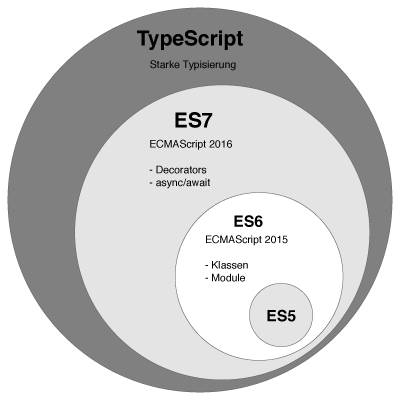
\includegraphics[width=0.5\linewidth]{JavaScript.png}
	\caption{Beziehung zwischen ECMAScript und TypeScript} 
	\quelle{\textcite[28]{Woiwode.2018}}
	\label{fig:ECMAScript}
\end{figure}

\subsection{Die Obermenge TypeScript}
TypeScript ist eine von Anders Hejlsberg bei Microsoft entwickelte Sprache. Diese erweitert die bestehende ECMAScript Version um weitere Sprachelemente und bildet somit eine Obermenge von JavaScript (siehe \autoref{fig:ECMAScript}). Ein Transpilierer übersetzt TypeScript in JavaScript. 

TypeScript ergänzt JavaScript unter anderem um ein stärkeres Typsystem. Hierdurch können Typfehler bereits zur Compilezeit erkannt und Tools zur Codeanalyse (automatische Codevervollständigung, Refactoring-Unterstützung, …) eingesetzt werden.\autocites[vgl.][27\psqq]{Woiwode.2018}[vgl.][13\psqq]{Steyer.2017}[vgl.][10]{Zeigermann.2016} Folgende Basistypen stellt TypeScript zur Verfügung: \autocites[vgl.][34\psqq]{Woiwode.2018}[vgl.][16\psqq]{Steyer.2017}

\begin{itemize}
	\item  \textbf{number}: Ganz- oder Kommazahl
	\item \textbf{string}:  Zeichenkette
	\item \textbf{boolean}: Wahrheitswert
	\item \textbf{Array<typ>}: typisierte Arrays
	\item \textbf{any}: simuliert Standardverhalten von JavaScript  – beliebiger Datentyp
	\item \textbf{Function}: Funktion
\end{itemize}
TypeScript ermöglicht die Verwendung von Interfaces. \autocites[vgl.][40\psq]{Woiwode.2018}

\subsection{Die Erweiterung JSX}\label{sec:die-erweiterung-jsx}
\label{Babel}
Die Spracherweiterung JSX ermöglicht die Verwendung einer HTML ähnlichen Syntax in JavaScript. JSX wird durch einen geeigneten Transpilierer in gültiges JavaScript übersetzt.\textcite[vgl.][10]{Zeigermann.2016} empfiehlt an dieser Stelle die Verwendung des Compilers \textit{Babel}.

Die Spracherweiterung kann zum Beispiel bei der Entwicklung mit dem Framework React eingesetzt werden. Dieses Framework verwendet zur Darstellung der Benutzeroberfläche keine Templatesgesetzt. Die Benutzeroberfläche wird stattdessen mitin icht unter Verwendung eines Templates, sondern üann JSX verwendet wrdenDie Verwendung von JSX Ausdrücken anstatt JavaScript-Befehlen erleichtert diesen Vorgang. Im Folgenden werden die Grundkonzept
Die Ausgabe von dynamische Informationen erfolgt unter Verwendung von JavaScript-Ausdrücken. Diese Ausdrücke müssen in ein paar geschweifter Klammern gepackt werden. Bedingungen können mithilfe des ternären Operatoren überprüft werden. Zur Ausgabe von Listen mit wiederholenden Elementen steht die für Arrays definierte JavaScript Methode map zur Verfügung.

JSX bietet zudem die Möglichkeit das Aussehen eines Elements über das style-Attribut zu verändern. Das sytle-Attribut ist ein Objekt, daher wird die CSS-Eigenschaft und der zugehörige Wert als Objekt-Literal übergeben. Zudem ist zu beachten, dass die CamelCase-Notation für die CSS-Eigenschaften verwendet werden muss. In \autoref{lst:JSXBeispiel} wird die CSS-Eigenschaft \textit{color} und \textit{font-size} des HTML-Elements gesetzt.

Um XSS-Attacken zu verhindern, werden Strings in JSX automatisch escaped bzw. maskiert. Ein String wird demnach immer als Text interpretiert und dargestellt.\autocites[vgl.][59\psqq]{Zeigermann.2016}[vgl.][65\psqq]{Stefanov.2017} 

\begin{lstlisting}[caption=Beispiel für die Verwendung von JSX, label=lst:JSXBeispiel, language=HTML]
const titleColor = 'red';
const titleFontSize = 12;
const helloWorld = <h1 style = {{
color: titleColor,
fontSize: titleFontSize + 'px'
}}> Hello, World</h1>
\end{lstlisting}


\comment{NodeJS}

\subsection{Zur Entwicklung benötigte Software oder Tools}
Für die Entwicklung einer auf JavaScript basierenden Webanwendung wird unter anderem NodeJS, der Paketmanager npm und ein Modul-Loader benötigt. Da diese Tools auch bei der Verwendung der Frameworks Angular und ReactJS eine Rolle Spielen, werden diese  im folgenden näher erläutert.
\section{Zur Entwicklung benötigte Tools}
Für die Entwicklung einer auf JavaScript basierenden Webanwendung wird unter anderem NodeJS, der Paketmanager npm und ein Modul-Loader benötigt. Demnach werden diese auch bei Verwendung der Frameworks Angular und ReactJS eingesetzt. Im Folgenden werden die Tools näher erläutert.

%NodeJS
\label{NodeJS}
Die JavaScript Laufzeitumgebung \textit{NodeJS} ermöglicht unter anderem das Ausführen von JavaScript Code auf dem Server. Einige Tools, die bei der Entwicklung einer Webanwendung eingesetzt werden, verwenden NodeJS. Außerdem bietet NodeJS Pakete mit wiederverwendbarem Code, die über den in integrierten Paketmanager \textit{npm} installiert werden können. Die aktuellste Version kann von \url{https://nodejs.org/} heruntergeladen und installiert werden.  \autocites[vgl.][1\psqq]{Steyer.2017}[vgl.][7\psqq]{Freeman.2018}[vgl.][6\psqq]{Woiwode.2018} 

\label{Webpack}
%Modul-Loader
Wenn Java-Script Module in einer Webanwendung verwendet werden, wird ein Modul-Loader gebraucht. Dieser löst verschiedene Abhängigkeiten auf und erstellt daraus eine Ausgabedatei. Die Verwendung des Modul-Loader \textit{Webpack} wird sowohl für Angular als auch für React Anwendungen empfohlen. \textit{Webpack} unterstützt zudem Hot Module Replacement. Änderungen am Code werden zur Laufzeit übernommen. Dadurch muss eine Anwendung nach einer Änderung nicht komplett neu gebaut werden.\autocites[vgl.][13,21]{Woiwode.2018}[vgl.][9,295-301]{Zeigermann.2016}[vgl.][]{Hlushko.2018}

